\chapter{Estado del arte}\label{cap:estado}

En esta sección se presenta una revisión del estado del arte en el ámbito de la planificación y gestión de horarios académicos, así como las tecnologías y paradigmas arquitectónicos utilizados en el desarrollo de sistemas de información basados en web. Se analizarán las limitaciones de los sistemas actuales, se compararán con soluciones más avanzadas implementadas en otras instituciones, y se explorarán las tecnologías y stacks utilizados en el desarrollo del sistema propuesto.

\section{Contextualización}

La planificación temporal y académica son pilares indispensables para un buen desempeño en el entorno universitario. Para los alumnos de centros con una estructura académica compleja, o profesores con varias horas de docencia en diferentes grupos, como la Escuela Técnica Superior de Ingenierías Informática y de Telecomunicación (ETSIIT) de la Universidad de Granada (UGR), o incluso varios grados, la capacidad de organizar y visualizar sus horarios de manera clara y personalizada se convierte en una necesidad notable.
\newline\newline
La gestión de múltiples asignaturas, grupos de teoría y prácticas, seminarios, tutorías y actividades personales requiere de herramientas que vayan más allá de la simple presentación estática de información, y además de manera general para toda la institución.
\newline\newline
Sin embargo, los sistemas tradicionales de visualización de horarios en muchas instituciones académicas presentan limitaciones significativas. De manera frecuente, la información se ofrece en formatos estáticos, como documentos PDF o imágenes, que dificultan la personalización, la interacción, la integración con las herramientas digitales que los estudiantes utilizan en su día a día, y en algunos casos una visibilidad accesible.
\newline\newline
Esta falta de dinamismo y personalización puede generar confusión, dificultar la planificación y no aprovechar las ventajas que ofrecen las tecnologías actuales para una gestión académica más eficiente y adaptada a las necesidades individuales.
\newline\newline
Este capítulo presenta una revisión del estado del arte que fundamenta la necesidad y el enfoque del proyecto. Se analiza la situación actual de la gestión y visualización de horarios en la UGR. 
Posteriormente, se realizará un análisis comparativo con sistemas más avanzados implementados en otras instituciones de educación superior. A continuación, se profundizará en los paradigmas arquitectónicos de backend y en tecnologías en el desarrollo de sistemas de información basados en web. Finalmente, se examinarán los diferentes stacks tecnológicos, incluyendo Java y el ecosistema Spring para el desarrollo de microservicios, RabbitMQ para la comunicación asíncrona, la combinación de bases de datos MySQL y MongoDB bajo el principio de persistencia políglota, la librería Jsoup para la adquisición de datos mediante web scraping, y las tecnologías empleadas para el despliegue del sistema, como Docker.

\section{Visualización y gestión de horarios académicos en la UGR}

La Universidad de Granada, al igual que muchas otras universidades, descentraliza sus sedes, de modo que
cada una de ellas tiene su propio sistema de gestión de la información. En este sentido, las facultades cuentan
con una serie de sistemas de información propios que se encargan de la generación de horarios académicos,
asignación de aulas y profesores a los grupos tanto de teoría como de prácticas 
de las distintas titulaciones y asignaturas. Esta información a su vez se le facilita a la Universidad de Granada para la centralización de la información.
\newline\newline
Para acceder a la información de los horarios, los estudiantes y docentes pueden hacerlo de diferentes maneras:
\begin{itemize}
    \item A través de la página propia de su facultad. Poniendo de ejemplo a la ETSIIT, debemos acceder a la página oficial de la facultad \cite{webETSIIT} y buscar la información en la sección
          de ``Calendario de exámenes`` en caso de querer saber los días y rangos horarios de estos y visualizándolo con un pdf, o a ``Calendario académico y horarios`` y a ``Grado en Ingeniería Informática``
          en caso de querer saber los horarios de los diferentes grupos del grado, presentado todo ello en un pdf contenedor de alrededor de 40 tablas.
          \newline\newline
          De esta manera tendremos que buscar el año al que pertenece la asignatura de la que estamos matriculados y el grupo al que pertenecemos. De esta manera obtenemos su 
          franja horaria y aula, pero no profesor que imparte la asignatura.
          \newline\newline
          Sin embargo, el formato de las tablas cambia de un grado a otro~\ref{fig:horarios_comparacion}, haciendo que el estudiante tenga que buscar la información de manera diferente en cada grado si está matriculado en más de uno, 
          y obteniendo información diferente. En el caso del grado de Administración y Dirección de Empresas por ejemplo, no se muestra el aula en la que se imparte la clase, pero sí las asignaturas bilingües, y
          los profesores que las imparten.
          \newline\newline
          Esta forma de visualización de horarios es inconsistente entre grados, y no es accesible para personas con discapacidad visual.
          %% Comparación de horarios de diferentes grados ( 2 imágenes )
          %% Como se insertan dos imagenes en latex con un unico pie de foto -> 
          \newpage
            \begin{figure}[H]
                \centering
                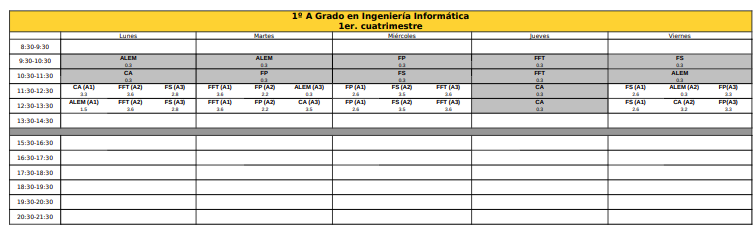
\includegraphics[width=0.8\textwidth]{figures/02_etsiit_horario.png}
                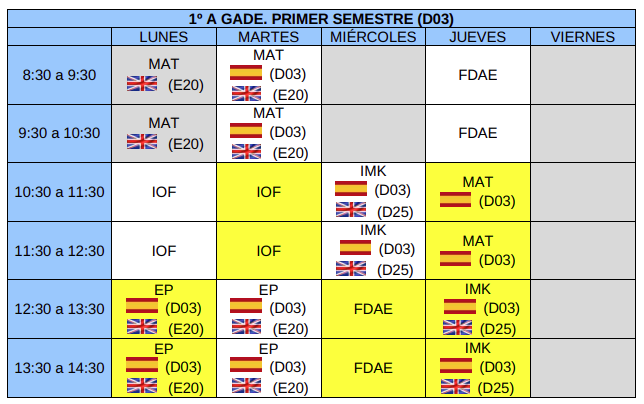
\includegraphics[width=0.8\textwidth]{figures/02_ade_horario.png}
                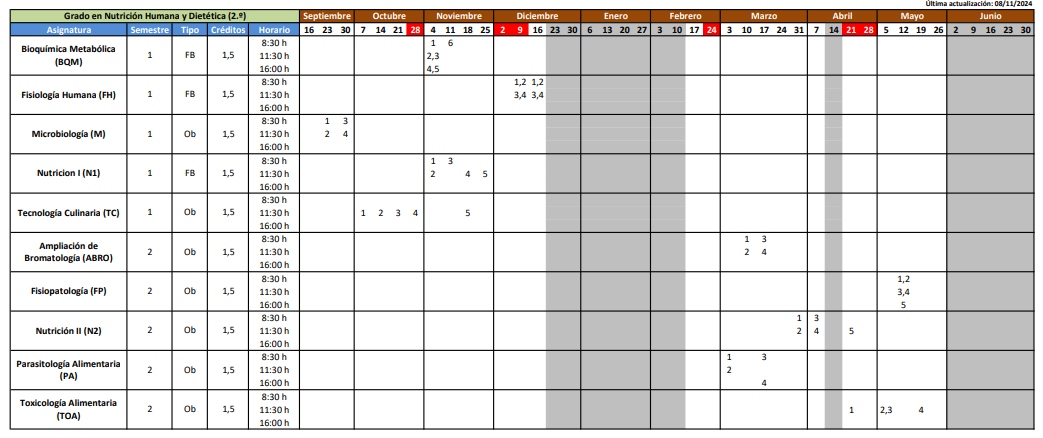
\includegraphics[width=0.8\textwidth]{figures/02_horario_doble_grado.png}
                \caption{Comparación de horarios de diferentes grados: ETSIIT (arriba), ADE (centro) y Doble Grado en Nutrición Humana y Dietética (abajo).}
                \label{fig:horarios_comparacion}
            \end{figure}
          

    \item A través de la web grados UGR \cite{webGrados} se puede buscar la información de los horarios de las asignaturas de los diferentes grados de la Universidad de Granada. Para ello debemos seleccionar rama de conocimiento, 
          grado, curso y asignatura. De esta manera obtenemos un horario semanal con las franjas horarias, aulas, profesores y fechas tanto de inicio como de fin. Este método nos proporcionan una interfaz estándar y más información, pero 
          también es más lento y tedioso para consultar por varias asignaturas o incluso grados.
    \item A través de las webs de cada departamento. Por ejemplo en la web del departamento de Ciencias de la Computación e Inteligencia Artificial \cite{webDecsai} se puede consultar la información de las asignaturas o profesores de este.
          Ofrece información adicional como asignaturas que imparte ``x'' profesor y su horario de tutorías y docencia.
\end{itemize}

Además para acceder a la información de periodos de actividad docente, exámenes finales, periodos de evaluación de convocatorias ... se ha de acceder a la web de la Secretaría General en la UGR \cite{webSecretaria} para consultar otro pdf.

En general la información de los horarios académicos de la Universidad de Granada es poco accesible, eficiente y consistente entre grados y facultades, lo que hace que el estudiante tenga que buscar la información de manera manual y tediosa.
Además no hay manera de consultar de manera sencilla un calendario personal que incluya tanto los horarios de las asignaturas como los exámenes y periodos de evaluación, entre otros.
\newline\newline
Pongamos el ejemplo de un estudiante matriculado en el primer curso del Grado de Biología en la Universidad de Granada con el estándar de cinco asignaturas en su primer cuatrimestre~\ref{fig:horario_biologia}. 
Este estudiante tiene que buscar la información de los horarios de las asignaturas en la web de su facultad, en la web de la Universidad de Granada o en la web del departamento al que pertenezca cada asignatura.
Suponemos que decide buscar su horario en la web de grados ugr, y una vez seleccionada la rama de conocimiento, grado, curso y asignatura, obtiene un horario semanal con las franjas horarias de todos los grupos de la asignatura, aulas, profesores y fechas tanto de inicio como de fin.
Está matriculado por ende en la asignatura ''Bases Químicas de la Biología'' en el grupo ``A'' de teoría y en el grupo ``2'' de prácticas, por lo que tiene que buscar los sectores que pertenecen a su grupos para poder obtener su horario personalizado para esa materia.
\newline\newline
La realidad con la que se encuentra el estudiante es con la siguiente:

\begin{figure}[H]
    \centering
    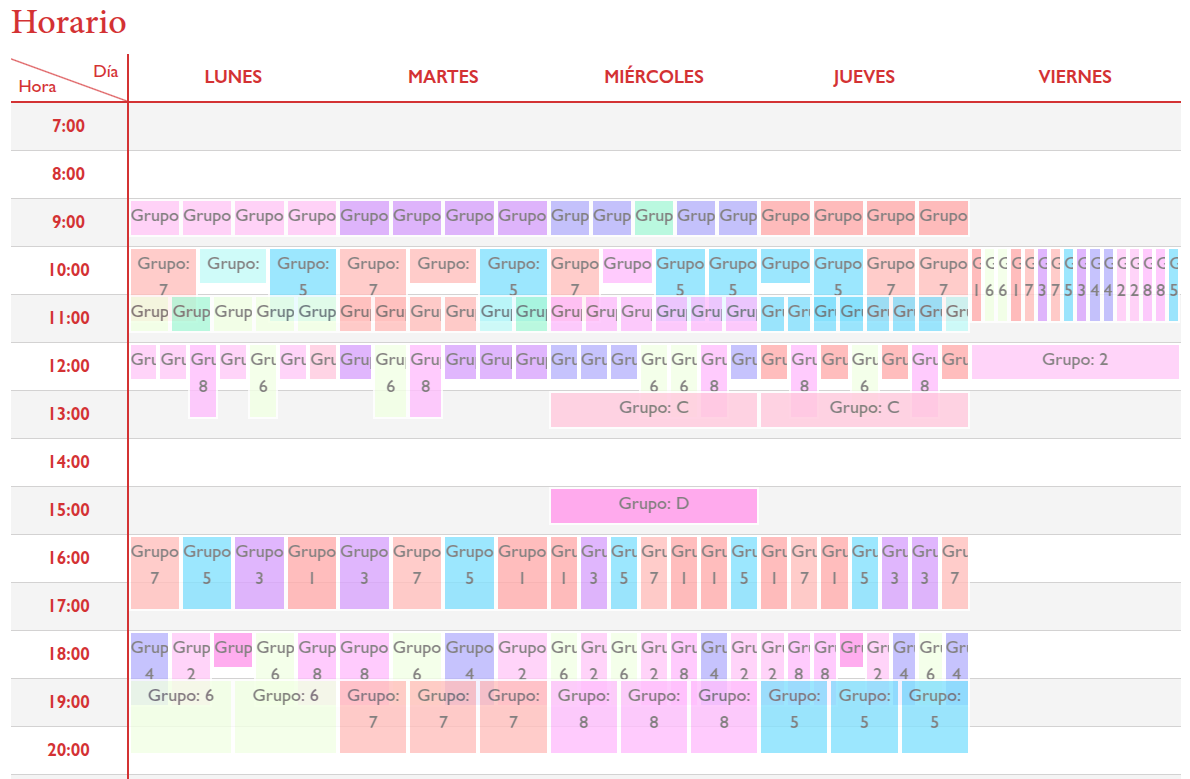
\includegraphics[width=0.8\textwidth]{figures/02_horario_biologia.png}
    \caption{Horario de la asignatura Bases Químicas de la Biología, impartida en el Grado en Biología.}
    \label{fig:horario_biologia}
\end{figure}

El estudiante tiene que dedicar un tiempo considerable en buscar las franjas pertenecientes a sus grupos, puesto que no hay una sencilla visualización de los mismos. Además se requiere una búsqueda activa con el cursor
para poder ver las franjas ocultas, y esta acción puede resultar tediosa cuando hay muchos sectores juntos, como en este caso.

Podemos concluir tras analizar la situación actual de aprovisionamiento de horarios académicos a los usuarios de la Universidad de Granada, que surge la necesidad de un sistema que permita la visualización de horarios académicos de manera sencilla, accesible y personalizada.

\section{Análisis comparativo de sistemas de planificación personalizada en educación superior}

Frente al modelo estático observado de manera generalizada en la Universidad de Granada, el panorama de la gestión de horarios en otras instituciones de educación superior y en el mercado de software educativo muestra una clara tendencia hacia sistemas más dinámicos, personalizados e integrados. 
\newline\newline
Existen diversas soluciones, desde módulos dentro de grandes sistemas ERP educativos hasta herramientas especializadas en la creación y gestión de horarios y planificadores académicos, pasando por aplicaciones de seguimiento del tiempo adaptadas al ámbito educativo.
El análisis de estas herramientas revela un conjunto de características comunes y avanzadas que definen el estado del arte en este dominio:

\begin{itemize}
      \item Por un lado ciertas universidades han desarrollado sistemas internos que permiten a los estudiantes acceder a sus horarios de manera personalizada, integrando información sobre asignaturas, grupos, aulas y profesores. Estos sistemas suelen ofrecer una interfaz gráfica intuitiva y accesible,
      permitiendo a los usuarios visualizar su horario de manera clara y sencilla. 

      %% 2 jpeg one next to the other

      \begin{figure}[H]
            \centering
            \makebox[\textwidth][c]{%
                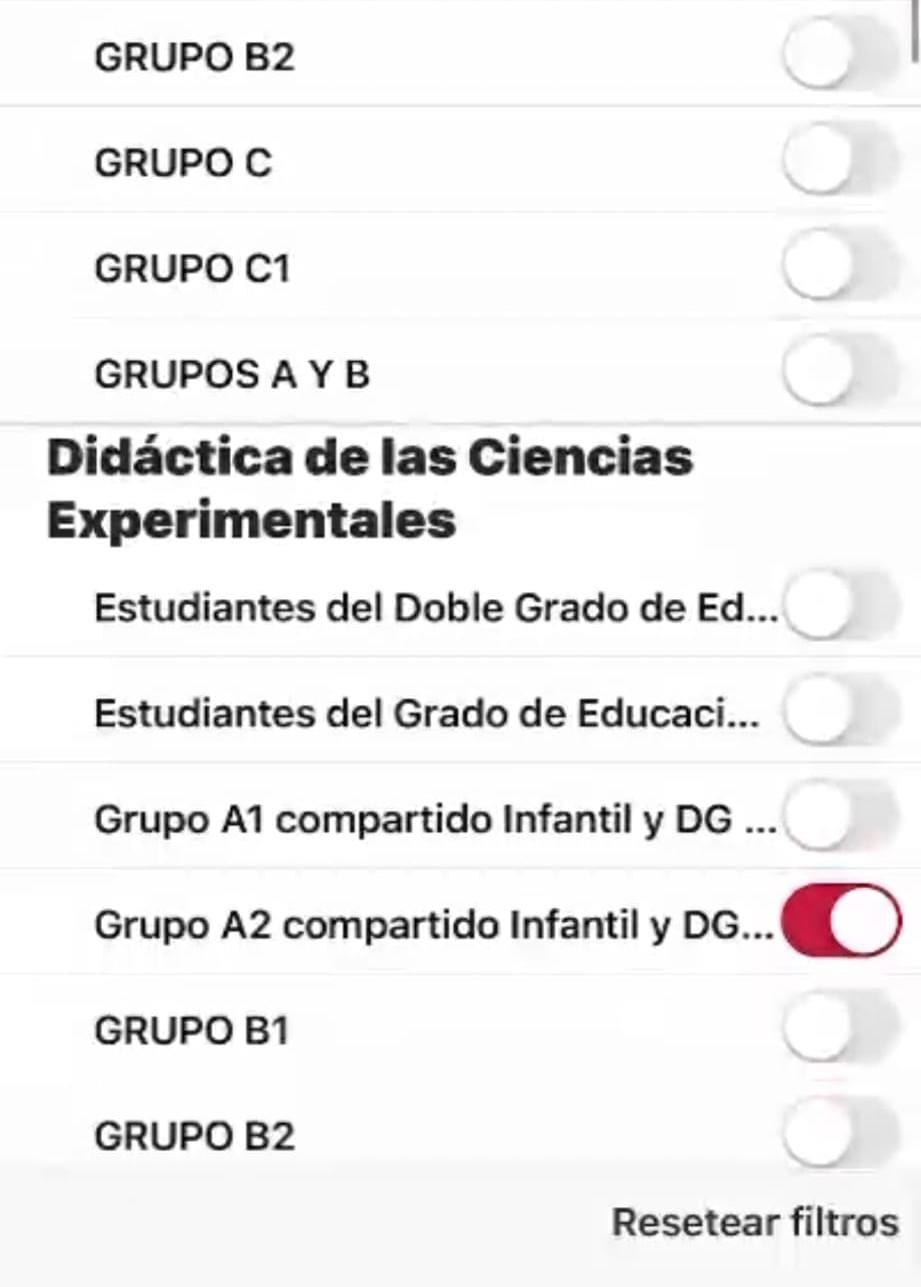
\includegraphics[height=8cm]{figures/03_ual_app_filtros.jpeg}
                \hspace{2cm}
                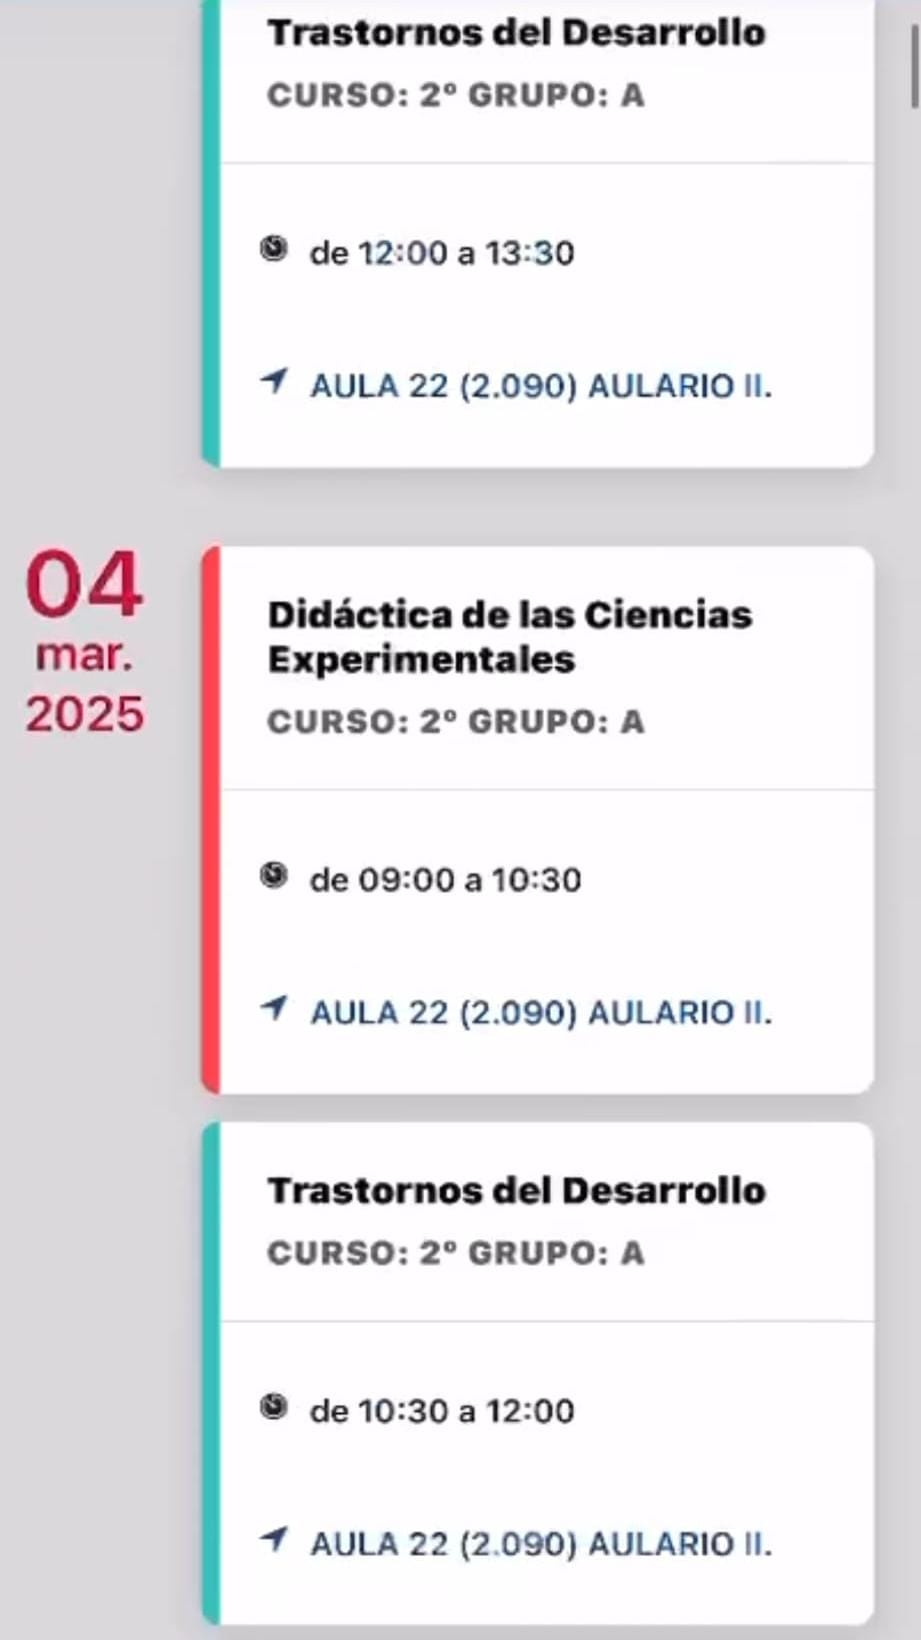
\includegraphics[height=8cm]{figures/03_ual_app_horarios.jpeg}
            }
            \caption{Aplicación móvil de la Universidad de Almería (UAL App).}
            \label{fig:ual_app}
        \end{figure}

      Exponiendo un ejemplo, la Universidad de Almería (UAL) ha implementado en su aplicación móvil multiplataforma ``UAL App''~\ref{fig:ual_app}, la posibilidad de, seleccionando las asignaturas y grupos en los que se está matriculado, obtener
      una lista de las actividades ordenadas por hora según el día de la semana.
      \newline
      De esta manera en la misma aplicación que los estudiantes usan para consultar sus notas, expediente académico, días festivos, etc. pueden consultar su horario académico de manera rápida en el mismo ecosistema.

      \item Por otro lado, y de manera externa a las universidades, existen aplicaciones de gestión de horarios y planificación personal que permiten a los estudiantes integrar sus horarios académicos con otras actividades personales, como trabajos, eventos sociales o compromisos familiares. 
      \newline\newline
      Estas aplicaciones suelen ofrecer funciones avanzadas de recordatorios, notificaciones y sincronización con calendarios digitales, lo que facilita la organización del tiempo y la gestión de tareas.
      Un ejemplo representativo de este tipo de sistemas es 'My Study Life' \cite{webMyStudyLife}, una aplicación multiplataforma que permite a los estudiantes gestionar sus horarios académicos, tareas y exámenes de manera integrada~\ref{fig:mystudylife}. En este caso el sistema en sí no cuenta con los datos internos de la universidad, sino que el estudiante tiene que introducir manualmente los datos de sus asignaturas y grupos, sin embargo, ofrece una interfaz intuitiva y fácil de usar, permitiendo a los estudiantes visualizar su horario de manera clara y sencilla.
      Además de la posibilidad de añadir tareas y exámenes, la aplicación permite establecer recordatorios y notificaciones para ayudar a los estudiantes a mantenerse organizados y cumplir con sus plazos, y es posee widgets personalizados para la pantalla de inicio de los dispositivos móviles e incluso aplicaciones para smartwatch, lo que consigue una integración total con el ecosistema del usuario.

      \begin{figure}[H]
            \centering
            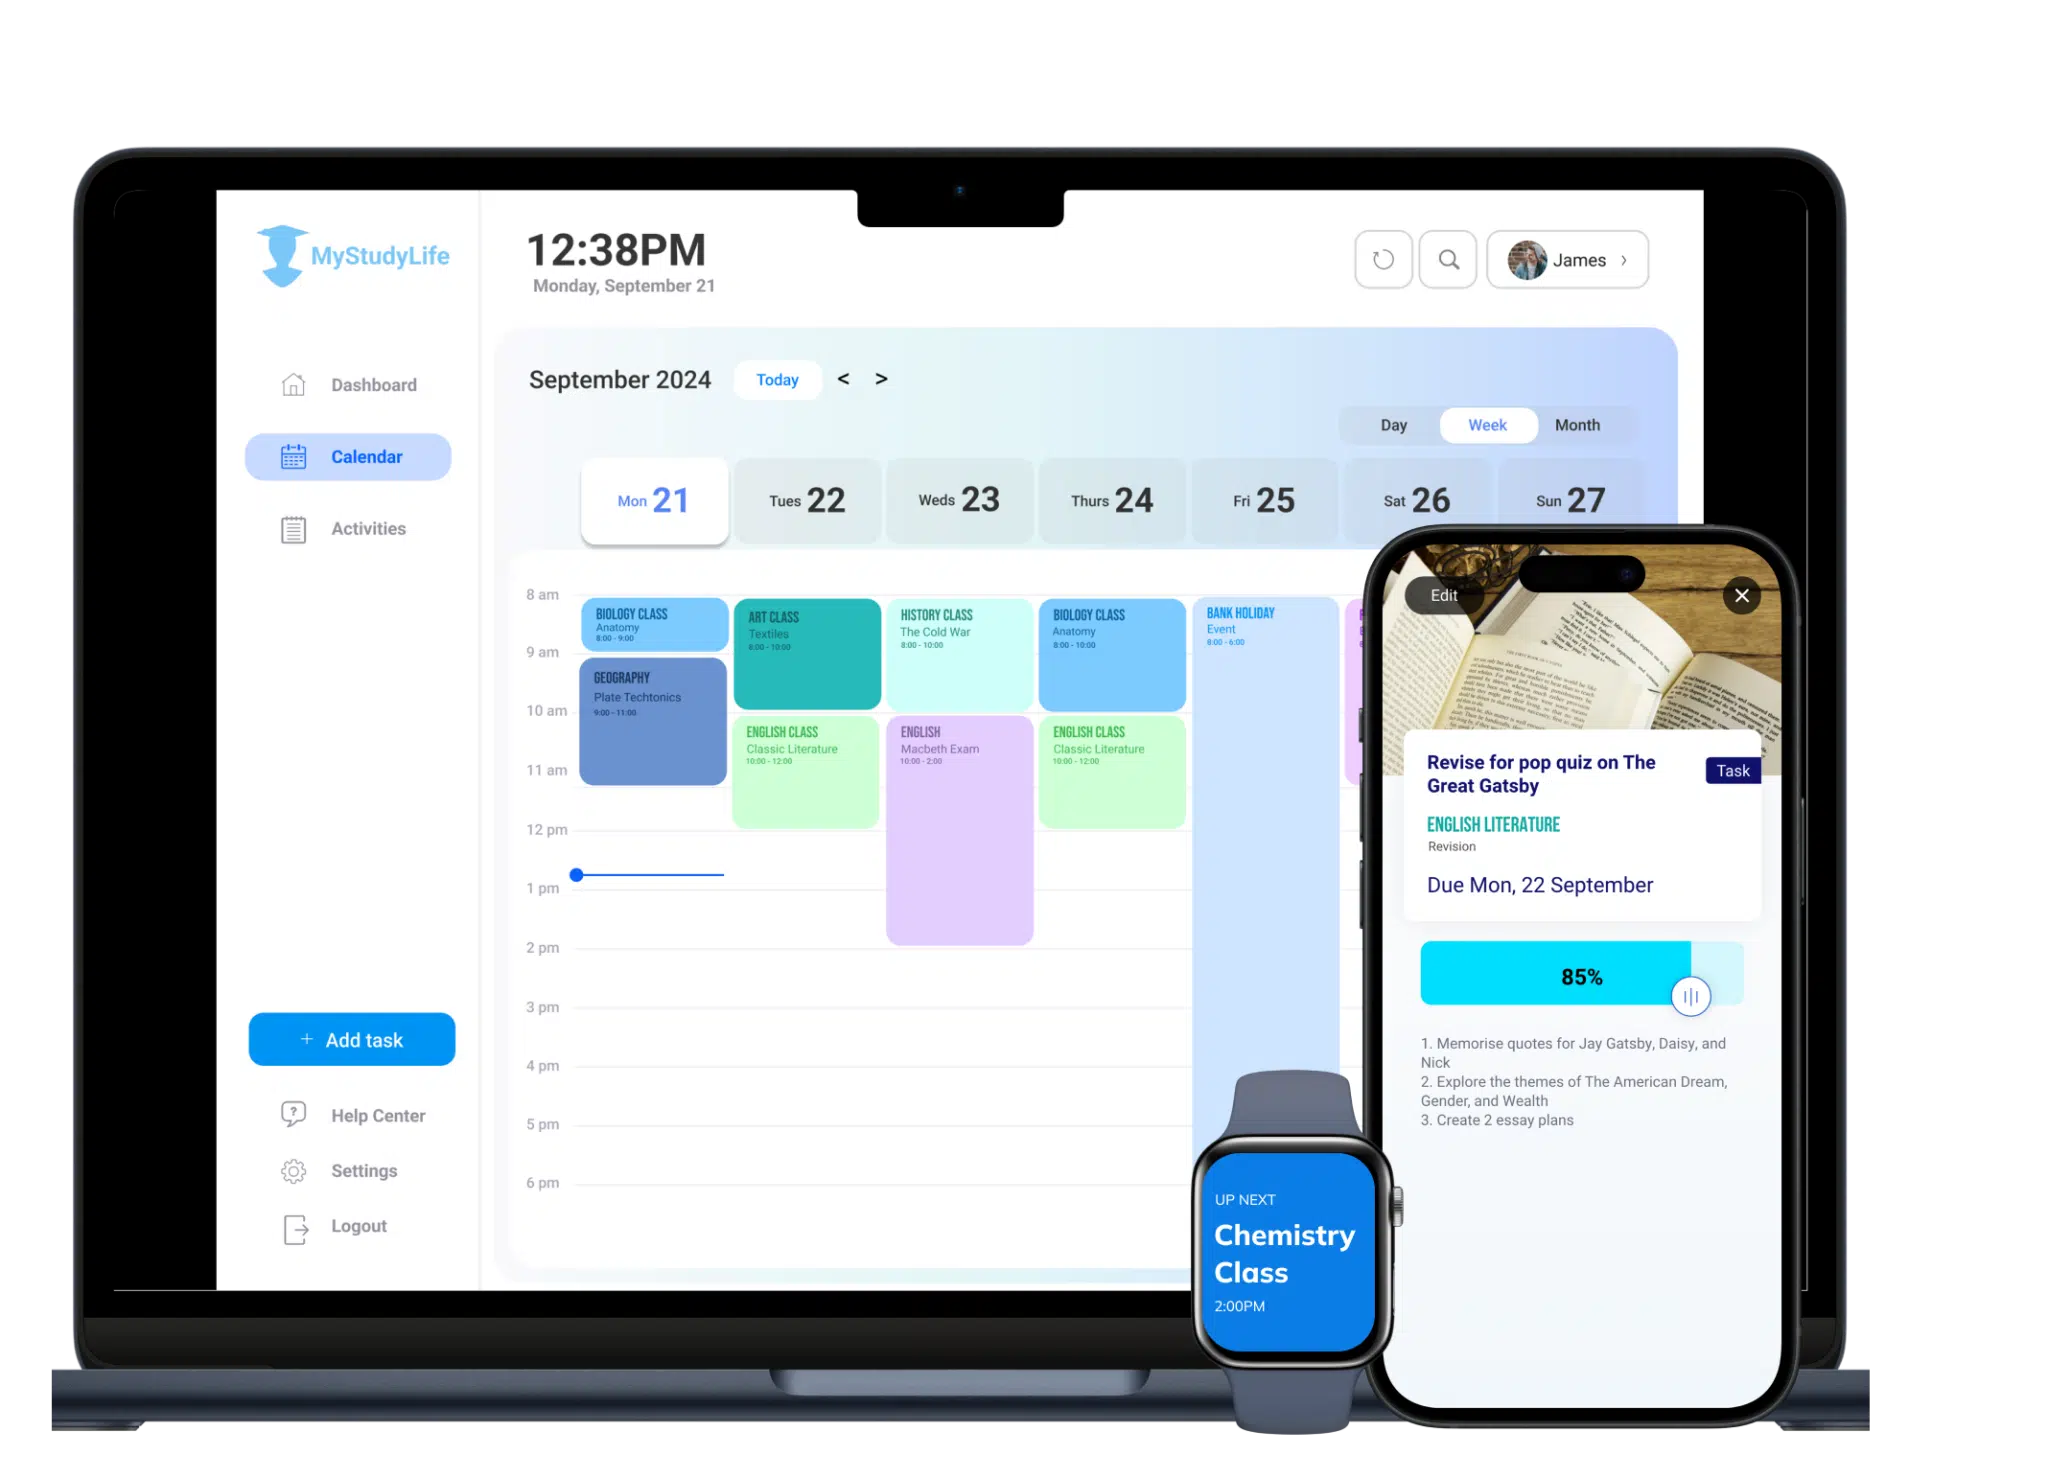
\includegraphics[width=0.8\textwidth]{figures/03_my_study_life.png}
            \caption{Aplicación My Study Life.}
            \label{fig:mystudylife}
      \end{figure}

      De manera general, y de uso más extendido, existen aplicaciones de gestión de tiempo y productividad que permiten a los usuarios organizar su tiempo de manera más eficiente como lo son Google Calendar \cite{webGoogleCalendar} o Microsoft Outlook \cite{webOutlook}.
      Estas aplicaciones permiten a los usuarios crear eventos, establecer recordatorios y sincronizar sus calendarios con otros dispositivos y aplicaciones. Sin embargo, no están específicamente diseñadas para la gestión de horarios académicos y pueden carecer de algunas funciones avanzadas que ofrecen otras aplicaciones más especializadas.
      Sin embargo también son usados para, sincronizando calendarios de sistemas externos, centralizar la información de los horarios académicos y otras actividades personales en un solo lugar, lo que facilita la gestión del tiempo y la planificación de tareas.

      \item Por último, existen sistemas de gestión de horarios y planificación académica que se integran con plataformas de aprendizaje en línea y sistemas de gestión del aprendizaje \hyperlink{lms}{LMS}, como Moodle \cite{webMoodle} o Blackboard.
      Estos sistemas permiten a los estudiantes acceder a su horario académico y a la información relacionada con sus cursos de manera centralizada, facilitando la gestión de tareas, exámenes y actividades académicas.
      Un ejemplo de este tipo de sistemas es el módulo de planificación académica de Moodle que permite a los estudiantes visualizar su horario académico y gestionar sus tareas y exámenes de manera integrada con la plataforma de aprendizaje.
      \newline\newline
      Este módulo ofrece una interfaz gráfica intuitiva y accesible, permitiendo a los estudiantes personalizar su horario académico y acceder a la información relacionada con sus cursos de manera centralizada. Además, el módulo de planificación académica de Moodle permite a los estudiantes establecer recordatorios y notificaciones para ayudarles a mantenerse organizados y cumplir con sus plazos.
      \newline\newline
      Sin embargo, este tipo de sistemas suelen estar limitados a las plataformas de aprendizaje en línea y no ofrecen la misma flexibilidad y personalización que otras aplicaciones de gestión de horarios y planificación personal.

\end{itemize}

\section{Desarrollo de servicios web}\label{sec:desarrollo_servicios_web}

El desarrollo de servicios web ha evolucionado significativamente en los últimos años, impulsado por la creciente demanda de aplicaciones distribuidas y la necesidad de integrar sistemas heterogéneos. En este contexto, se han desarrollado diferentes paradigmas arquitectónicos y tecnologías que permiten la creación de servicios web eficientes y escalables.

Esta evoluci\'{o}n ha llevado a una clara distinci\'{o}n de responsabilidades en el desarrollo de aplicaciones web, consolidando los conceptos de \hyperlink{frontend}{Frontend} y \hyperlink{backend}{Backend} como pilares fundamentales.

El \textbf{frontend}, tambi\'{e}n conocido como el "lado del cliente", es la parte de la aplicaci\'{o}n con la que el usuario interact\'{u}a directamente. Abarca la interfaz de usuario (\hyperlink{ui}{UI}), la experiencia de usuario (\hyperlink{ux}{UX}) y toda la l\'{o}gica que se ejecuta en el navegador web del cliente. Las tecnolog\'{i}as predominantes en el desarrollo frontend incluyen HTML para la estructura, CSS para la presentaci\'{o}n y JavaScript para la interactividad. 
\newline\newline
En los \'{u}ltimos a\~{n}os, frameworks y bibliotecas de JavaScript como React, Angular y Vue.js han ganado una enorme popularidad, permitiendo la creaci\'{o}n de interfaces de usuario din\'{a}micas, complejas y reutilizables. Estos frameworks facilitan la gesti\'{o}n del estado de la aplicaci\'{o}n en el cliente y la comunicaci\'{o}n as\'{i}ncrona con el servidor, mejorando la fluidez y la reactividad de las aplicaciones web modernas.

Por otro lado, el \textbf{backend}, o "lado del servidor", es el motor que impulsa la aplicaci\'{o}n. Se encarga de la l\'{o}gica de negocio, el procesamiento de datos, la autenticaci\'{o}n de usuarios, la gesti\'{o}n de bases de datos y la comunicaci\'{o}n con otros sistemas o servicios. Es invisible para el usuario final, pero crucial para el funcionamiento de la aplicaci\'{o}n. Existe una amplia variedad de lenguajes y frameworks para el desarrollo backend, como Node.js (con Express.js o NestJS), Python (con Django o Flask), Java (con Spring), Ruby (con Ruby on Rails), PHP (con Laravel o Symfony) y C\# (con .NET). La elecci\'{o}n de la tecnolog\'{i}a backend suele depender de factores como los requisitos de rendimiento, la escalabilidad, la experiencia del equipo de desarrollo y el ecosistema existente. El backend tambi\'{e}n es responsable de la seguridad de la aplicaci\'{o}n, implementando medidas para proteger los datos y prevenir accesos no autorizados.

La comunicaci\'{o}n entre el frontend y el backend se ha estandarizado en gran medida a trav\'{e}s de las \textbf{Interfaces de Programaci\'{o}n de Aplicaciones (\hyperlink{api}{API})}. 

Las Apis son vitales para la creación de experiencias digitales modernas, ya que simplifican como los sistemas se comunican, ofreciendo flexibilidad e independencia a una empresa. El mundo de las APIs está en constante evolución, y cada vez más empresas están adoptando este enfoque para integrar sus sistemas y servicios. Las APIs permiten a los desarrolladores acceder a funcionalidades específicas de una aplicación o servicio sin necesidad de conocer su implementación interna, lo que facilita la creación de aplicaciones complejas y la integración de diferentes sistemas.
\newline
Son cuatro tecnologías las que se han estandarizado como las más utilizadas para la creación de APIs: REST, SOAP, GraphQL y gRPC.

\begin{enumerate}
    \item \textbf{\hyperlink{rest}{REST} - El Estándar Atemporal}
    \begin{itemize}
        \item \textbf{Ventajas:} Maduro y ampliamente adoptado, simple y flexible, sin estado, múltiples tipos de medios.
        \item \textbf{Limitaciones:} Sobre-recuperación y sub-recuperación, complejidad de versionado, capacidades de tiempo real limitadas.
        \item \textbf{Mejores Casos de Uso:} APIs públicas, operaciones CRUD simples, requisitos de tiempo real limitados.
        \item \textbf{Consideraciones:} Versionado y escalabilidad para grandes bases de usuarios, impacto de la sobre/sub-recuperación.
    \end{itemize}

    \item \textbf{\hyperlink{soap}{SOAP} - El Clásico Empresarial}
    \begin{itemize}
        \item \textbf{Ventajas:} Protocolo estandarizado, seguridad robusta (WS-Security), transacciones y confiabilidad.
        \item \textbf{Limitaciones:} Verbosidad, complejidad, menor flexibilidad que REST.
        \item \textbf{Mejores Casos de Uso:} Sistemas empresariales, integraciones complejas, requisitos de seguridad estrictos.
        \item \textbf{Consideraciones:} Complejidad del protocolo y herramientas, justificación del uso frente a REST.
    \end{itemize}

    \item \textbf{\hyperlink{graphql}{GraphQL} - El Orquestador Dinámico}
    \begin{itemize}
        \item \textbf{Ventajas:} Obtención de datos impulsada por el cliente (reduce la sobre-recuperación), relaciones de datos complejas eficientes, actualizaciones en tiempo real (subscriptions), esquema flexible.
        \item \textbf{Limitaciones:} Mayor complejidad del servidor, curva de aprendizaje, ecosistema de herramientas en evolución.
        \item \textbf{Mejores Casos de Uso:} Aplicaciones de una sola página (SPAs), estructuras de datos complejas, actualizaciones y suscripciones en tiempo real.
        \item \textbf{Consideraciones:} Complejidad del servidor e impacto en el rendimiento, documentación y herramientas para desarrolladores.
    \end{itemize}

    \item \textbf{\hyperlink{grpc}{gRPC} - El Conducto de Alto Rendimiento}
    \begin{itemize}
        \item \textbf{Ventajas:} Alto rendimiento (HTTP/2, Protocol Buffers), soporte de streaming, fuertemente tipado, herramientas maduras.
        \item \textbf{Limitaciones:} Curva de aprendizaje más pronunciada, menos flexible, adopción menos extendida.
        \item \textbf{Mejores Casos de Uso:} Comunicación entre microservicios de alto rendimiento, escenarios de streaming, operaciones intensivas en datos.
        \item \textbf{Consideraciones:} Complejidad de adopción de gRPC y Protocol Buffers, justificación del esfuerzo de desarrollo por las ganancias de rendimiento.
    \end{itemize}
\end{enumerate}

Las \textbf{APIs REST (Representational State Transfer)}, estrategia a seguir para la creación del backend del proyecto, se han convertido en el paradigma dominante para dise\~{n}ar estas interfaces debido a su simplicidad, escalabilidad y flexibilidad. Una API REST define un conjunto de reglas y convenciones para que los sistemas puedan comunicarse a trav\'{e}s del protocolo HTTP.

La creaci\'{o}n de una API REST que sirva al frontend implica varios pasos clave:

\begin{itemize}
    \item \textbf{Definici\'{o}n de Recursos:} Se identifican los recursos que la API expondr\'{a} (por ejemplo, usuarios, productos, pedidos). Cada recurso tiene una URI (Uniform Resource Identifier) \'{u}nica.
    \item \textbf{Uso de M\'{e}todos HTTP \cite{MDNHTTPMethods2025}:} HTTP define un conjunto de métodos de petición para indicar la acción que se desea realizar para un recurso determinado. Aunque estos también pueden ser sustantivos, estos métodos de solicitud a veces son llamados HTTP verbs. Cada uno de ellos implementan una semántica diferente, pero algunas características similares son compartidas por un grupo de ellos: ej. un request method puede ser safe, idempotent, o cacheable.
    \newline\newline
    Los más usados son :
    \begin{itemize}
        \item \texttt{GET}: Solicita una representación de un recurso específico. Las peticiones que usan el método GET sólo deben recuperar datos.
        \item \texttt{HEAD}: Similar a GET, pero no devuelve el cuerpo de la respuesta, solo los encabezados. Se utiliza para obtener metadatos.
        \item \texttt{POST}: Se utiliza para enviar una entidad a un recurso en específico, causando a menudo un cambio en el estado o efectos secundarios en el servidor.
        \item \texttt{PUT}: Reemplaza todas las representaciones actuales del recurso de destino con la carga útil de la petición.
        \item \texttt{PATCH}: Aplica modificaciones parciales a un recurso.
        \item \texttt{OPTIONS}: Describe las opciones de comunicación para el recurso de destino. Permite al cliente conocer las capacidades del servidor.
        \item \texttt{DELETE}: Borra un recurso en específico.
    \end{itemize}
    \item \textbf{Representaci\'{o}n de Datos:} Los datos intercambiados entre el cliente y el servidor suelen estar en formato JSON (JavaScript Object Notation) debido a su ligereza y facilidad de parseo por parte de los navegadores y la mayor\'{i}a de los lenguajes de programaci\'{o}n. XML tambi\'{e}n puede ser utilizado, aunque es menos com\'{u}n en APIs modernas orientadas a frontend.
    \item \textbf{Statelessness (Ausencia de Estado):} Cada petici\'{o}n del cliente al servidor debe contener toda la informaci\'{o}n necesaria para que el servidor la entienda y procese. El servidor no almacena ning\'{u}n estado de la sesi\'{o}n del cliente entre peticiones. Esto simplifica el dise\~{n}o del servidor y mejora la escalabilidad.
    \item \textbf{Uso de C\'{o}digos de Estado HTTP:} Se utilizan c\'{o}digos de estado HTTP para indicar el resultado de una petici\'{o}n (por ejemplo, \texttt{200 OK}, \texttt{201 Created}, \texttt{400 Bad Request}, \texttt{401 Unauthorized}, \texttt{404 Not Found}, \texttt{500 Internal Server Error}).
\end{itemize}

El backend desarrolla estos endpoints de la API REST, implementando la l\'{o}gica necesaria para cada operaci\'{o}n. El frontend, a su vez, realiza peticiones HTTP (utilizando APIs del navegador como \texttt{Fetch} o bibliotecas como Axios) a estas URLs para enviar y recibir datos, actualizando din\'{a}micamente la interfaz de usuario sin necesidad de recargar la p\'{a}gina completa. Este desacoplamiento entre frontend y backend permite que ambos puedan desarrollarse, probarse, desplegarse y escalarse de forma independiente, facilitando la colaboraci\'{o}n entre equipos y la adopci\'{o}n de diferentes tecnolog\'{i}as para cada capa. Adem\'{a}s, una API REST bien dise\~{n}ada puede servir no solo a una aplicaci\'{o}n web, sino tambi\'{e}n a aplicaciones m\'{o}viles u otros servicios, promoviendo la reutilizaci\'{o}n y la interoperabilidad entre sistemas heterog\'{e}neos, tal como se mencionaba al inicio.

La tendencia hacia arquitecturas de microservicios en el backend ha reforzado a\'{u}n m\'{a}s la importancia de las APIs REST bien definidas, ya que cada microservicio suele exponer su funcionalidad a trav\'{e}s de una API. En este contexto, herramientas como OpenAPI (anteriormente Swagger) para la definici\'{o}n y documentaci\'{o}n de APIs, y soluciones de API Gateway para la gesti\'{o}n, seguridad y monitorizaci\'{o}n del tr\'{a}fico de las APIs, se han vuelto indispensables en el desarrollo de servicios web modernos y robustos.

\subsection{Arquitecturas de software}

La elección de la arquitectura backend es una decisión fundamental en el desarrollo de cualquier aplicación web, impactando directamente en su escalabilidad, mantenibilidad, flexibilidad y velocidad de desarrollo. Para un sistema de gestión de horarios académicos como el propuesto, que potencialmente puede crecer en complejidad y número de usuarios, la comparación entre los enfoques monolítico y de microservicios es particularmente relevante.

Si bien la arquitectura monolítica ha sido tradicionalmente un punto de partida, la creciente complejidad de los sistemas y la necesidad de agilidad han impulsado la adopción y evolución de diversos paradigmas arquitectónicos. A continuación, se presenta una exposición de diferentes arquitecturas de software \cite{bookORellySoftwareArchitecture} implementadas en sistemas backend, analizando sus características y su posición en el espectro que va desde el monolito hasta los microservicios.

\subsubsection*{Arquitectura en Capas (Layered Architecture / N-Tier Architecture) \cite{clean_architecture}}

\begin{description}
    \item[\textbf{Descripción:}] Este es uno de los patrones arquitectónicos más establecidos y fundamentales. Consiste en la organización del código en capas horizontales, donde cada capa posee una responsabilidad específica y se comunica, por lo general, únicamente con las capas adyacentes (superior e inferior). Las capas típicas suelen ser:
    \begin{itemize}
        \item \textit{Capa de Presentación (o Interfaz de Usuario):} Gestiona la interacción con el usuario o sistemas cliente. En el contexto de un backend, esta capa a menudo se materializa como la API que gestiona las solicitudes HTTP.
        \item \textit{Capa de Aplicación (o Lógica de Negocio):} Contiene la lógica de negocio central y orquesta las tareas y flujos de trabajo.
        \item \textit{Capa de Dominio (o Modelo de Negocio):} Representa las entidades, los objetos de valor y las reglas inherentes al dominio del negocio.
        \item \textit{Capa de Acceso a Datos (o Persistencia):} Encargada de la comunicación con los sistemas de almacenamiento de datos, como bases de datos.
        \item \textit{Capa de Infraestructura:} Provee servicios técnicos transversales, tales como logging, monitorización, y comunicación de red.
    \end{itemize}
    \item[\textbf{Posicionamiento y Evolución:}] Una aplicación monolítica frecuentemente se estructura internamente siguiendo una arquitectura en capas. Aunque este patrón no descompone el sistema en servicios desplegables de forma independiente, sí promueve una modularización interna y una clara separación de responsabilidades (Separation of Concerns), lo cual es un primer paso crucial para gestionar la complejidad y facilitar la mantenibilidad de un sistema antes de considerar arquitecturas más distribuidas.
\end{description}

\subsubsection*{Arquitectura Orientada a Servicios (SOA - Service-Oriented Architecture) \cite{soa_ibm}}

\begin{description}
    \item[\textbf{Descripción:}] SOA es un paradigma de diseño que estructura una aplicación como una colección de servicios que se comunican entre sí. Estos servicios encapsulan funcionalidades de negocio discretas y pueden ser accedidos a través de la red. A menudo, los servicios en SOA son de grano más grueso en comparación con los microservicios. La comunicación se estandarizó frecuentemente mediante protocolos como SOAP (Simple Object Access Protocol) sobre HTTP, y es común el uso de un Enterprise Service Bus (ESB) para la mediación, el enrutamiento y la transformación de mensajes entre servicios.
    \item[\textbf{Características Clave:}] Fomenta la reutilización de servicios a nivel empresarial, la interoperabilidad entre sistemas heterogéneos y el descubrimiento dinámico de servicios.
    \item[\textbf{Posicionamiento y Evolución:}] SOA representó un avance significativo respecto a los monolitos, permitiendo una descomposición más formal y orientada a negocio. Puede considerarse un precursor importante de la arquitectura de microservicios. Sin embargo, SOA a menudo implicaba una mayor sobrecarga en términos de estándares, una gobernanza más centralizada y, en ocasiones, cuellos de botella debidos al ESB, aspectos que la arquitectura de microservicios busca simplificar o descentralizar.
\end{description}

\subsubsection*{Arquitectura Dirigida por Eventos (EDA - Event-Driven Architecture) \cite{aws_eda}}

\begin{description}
    \item[\textbf{Descripción:}] En una EDA, el flujo de la aplicación es determinado por la ocurrencia de eventos. Los eventos son notificaciones que representan un cambio de estado significativo o un suceso relevante dentro del sistema (por ejemplo, ``PedidoRealizado'', ``InventarioBajo''). Los componentes del sistema, denominados productores de eventos, publican estos eventos en un canal o bus de eventos (gestionado por un bróker de mensajes como Apache Kafka, RabbitMQ o Google Cloud Pub/Sub). Otros componentes, los consumidores de eventos, se suscriben a los eventos que les conciernen y reaccionan a ellos de forma asíncrona.
    \item[\textbf{Estilos Principales:}] Se distinguen dos topologías principales: el \textit{mediador de eventos}, donde un componente central orquesta el flujo de eventos, y el \textit{bróker de eventos}, que facilita una mayor desacoplamiento entre publicadores y suscriptores.
    \item[\textbf{Posicionamiento y Evolución:}] EDA es altamente compatible y a menudo se utiliza en conjunción con la arquitectura de microservicios para lograr una comunicación asíncrona, resiliente y escalable. Permite un desacoplamiento profundo entre servicios, mejorando la tolerancia a fallos y la capacidad de respuesta del sistema. También se emplea para modernizar sistemas monolíticos, permitiendo integrar nuevas funcionalidades de forma reactiva o desacoplar módulos existentes.
\end{description}

\subsubsection*{Arquitectura ``Serverless'' y Nativa de la Nube \cite{aws_serverless}}
\begin{description}
    \item[\textbf{Descripción:}] Este enfoque se centra en la ejecución de código sin necesidad de gestionar servidores o infraestructura subyacente. Los desarrolladores escriben funciones que se ejecutan en respuesta a eventos, y el proveedor de la nube (como AWS Lambda, Azure Functions o Google Cloud Functions) se encarga de la infraestructura, escalabilidad y disponibilidad. Las aplicaciones nativas de la nube están diseñadas para aprovechar al máximo las capacidades de la nube, como el escalado automático, la alta disponibilidad y los servicios gestionados.
    \item[\textbf{Características Clave:}] Despliegue basado en funciones, escalabilidad automática, pago por uso (se paga solo por el tiempo de ejecución), y enfoque en eventos y microservicios.
    \item[\textbf{Posicionamiento y Evolución:}] La arquitectura serverless es una evolución natural hacia una mayor abstracción y simplificación del desarrollo backend. Permite a los equipos centrarse en la lógica de negocio sin preocuparse por la infraestructura subyacente. Sin embargo, puede introducir desafíos relacionados con el estado, la latencia y el control sobre el entorno de ejecución.
    Este enfoque es especialmente adecuado para aplicaciones que requieren escalabilidad extrema y una alta disponibilidad, como sistemas de gestión de horarios académicos que pueden experimentar picos de carga durante períodos específicos (por ejemplo, al inicio del semestre).
\end{description}

\subsubsection*{Arquitectura de Microservicios \cite{ms_microservices}}

\begin{description}
    \item[\textbf{Descripción:}] Esta arquitectura estructura una aplicación como una suite de pequeños servicios independientes, cada uno enfocado en una capacidad de negocio específica y bien delimitada (Bounded Context). Cada microservicio es autónomo, lo que implica que puede ser desarrollado, desplegado, escalado y gestionado de forma independiente. Típicamente, cada servicio posee su propia base de datos para asegurar un bajo acoplamiento y se comunica con otros servicios a través de APIs ligeras y bien definidas, comúnmente utilizando HTTP/REST, gRPC, o a través de mensajería asíncrona.
    \item[\textbf{Características Clave:}] Despliegue independiente y continuo, escalabilidad granular (se escalan solo los servicios que lo necesitan), flexibilidad tecnológica (posibilidad de usar diferentes stacks tecnológicos por servicio), aislamiento de fallos (un fallo en un servicio no debería derribar todo el sistema), y alineación con equipos de desarrollo pequeños y autónomos (Conway's Law).
    \item[\textbf{Posicionamiento y Evolución:}] La arquitectura de microservicios se considera una evolución directa y una alternativa robusta para superar las limitaciones intrínsecas de los sistemas monolíticos, especialmente en contextos de alta complejidad, crecimiento rápido y necesidad de agilidad. Aborda desafíos como la dificultad para escalar, la complejidad en el mantenimiento, la lentitud en la adopción de nuevas tecnologías, los ciclos de despliegue prolongados y el alto acoplamiento que caracterizan a las grandes aplicaciones monolíticas.
\end{description}

\subsubsection*{Conclusión: Progresión y Criterios de Selección}

El panorama de arquitecturas backend ha evolucionado desde la simplicidad inicial de los sistemas \textbf{monolíticos}, pasando por la modularización interna de la \textbf{arquitectura en capas}, hacia la descomposición en servicios con \textbf{SOA}. Posteriormente, paradigmas como la \textbf{arquitectura dirigida por eventos} han ganado tracción para mejorar el desacoplamiento y la resiliencia, mientras que enfoques como la \textbf{arquitectura basada en el espacio} y los \textbf{principios nativos de la nube} abordan la escalabilidad extrema y la eficiencia en entornos cloud.

Finalmente, la \textbf{arquitectura de microservicios}, arquitectura a adoptar en el backend del sistema, emerge como un enfoque predominante para construir sistemas complejos, distribuidos y altamente escalables, ofreciendo un alto grado de agilidad y autonomía. No obstante, es crucial destacar que no existe una arquitectura universalmente superior. La selección de la arquitectura más adecuada debe ser el resultado de un análisis cuidadoso de los requisitos específicos del proyecto, el contexto del negocio, las capacidades del equipo de desarrollo, las proyecciones de escalabilidad y los compromisos (trade-offs) inherentes a cada patrón. En muchos sistemas del mundo real, es común encontrar combinaciones pragmáticas de estos patrones arquitectónicos.

\subsection{Tecnologías de desarrollo}

En el ámbito del desarrollo de software, la elección de las tecnologías adecuadas es crucial para el éxito de un proyecto. En este apartado, se presentan las principales tecnologías que se han considerado para el desarrollo del sistema de gestión de horarios académicos.

\subsubsection{Tecnologías y lenguajes backend}

\begin{enumerate}
    \item \textbf{Java con Spring Framework (Spring Boot y Spring Cloud)\cite{springcloud}:}
    Java es un lenguaje de programación robusto, maduro y ampliamente adoptado en el desarrollo de aplicaciones empresariales a gran escala. Su ecosistema es vasto, con una gran comunidad y un fuerte enfoque en el rendimiento y la seguridad. Spring Boot simplifica drásticamente la creación de aplicaciones basadas en Spring, ofreciendo auto-configuración, servidores web embebidos (como Tomcat o Jetty) y una gestión de dependencias simplificada, lo que lo convierte en una opción popular para el desarrollo rápido de microservicios listos para producción. De hecho, se considera el estándar de facto para microservicios en Java.

    Para arquitecturas de microservicios, Spring Cloud complementa a Spring Boot proporcionando un conjunto de herramientas y patrones para construir sistemas distribuidos resilientes y escalables. Esto incluye soluciones para el descubrimiento de servicios (permitiendo que los servicios se encuentren dinámicamente en la red), balanceo de carga (distribuyendo las solicitudes entre múltiples instancias de un servicio), pasarelas API (un punto de entrada único para todas las solicitudes de los clientes), interruptores de circuito (para prevenir fallos en cascada) y gestión de configuración distribuida. Dada la potencial complejidad de un sistema de gestión de horarios universitarios, especialmente si se opta por microservicios, la madurez y el soporte integral de Spring Cloud para estos patrones son altamente relevantes.

    \item \textbf{.NET Core\cite{dotnetcore}:}
    .NET Core (ahora parte de .NET 5 y versiones posteriores) es un framework de desarrollo de aplicaciones multiplataforma, de código abierto y de alto rendimiento mantenido por Microsoft. Es una opción sólida para construir microservicios, con excelente soporte para la creación de APIs RESTful, contenedores Docker y despliegue en plataformas de orquestación como Kubernetes. Ofrece características como escalabilidad, un modelo de entrega continua, herramientas para operaciones CRUD, soporte para comunicación síncrona y asíncrona entre servicios, y la implementación de patrones de diseño avanzados como CQRS (Command and Query Responsibility Segregation) y Event Sourcing. También se integra bien con tecnologías de caché como Redis y proporciona mecanismos de seguridad robustos mediante OAuth2 y OpenID Connect. Para equipos con experiencia en el ecosistema Microsoft o que buscan una alternativa de alto rendimiento a Java, .NET Core es una opción muy competente.

    \item \textbf{Node.js con Express.js\cite{expressjs}:}
    Node.js es un entorno de ejecución para JavaScript del lado del servidor, construido sobre el motor V8 de Chrome. Su principal característica distintiva es su modelo de E/S (Entrada/Salida) asíncrono y sin bloqueo, orientado a eventos. Esto lo hace particularmente eficiente para aplicaciones que manejan un gran número de conexiones concurrentes y operaciones de E/S intensivas, como aplicaciones en tiempo real o APIs que actúan como fachadas para otros servicios. Express.js es un framework web minimalista y flexible para Node.js, ampliamente utilizado para construir APIs RESTful y microservicios ligeros. Su simplicidad y el vasto ecosistema de paquetes disponibles a través de npm (Node Package Manager) permiten un desarrollo rápido. En el contexto de un sistema de gestión de horarios, Node.js con Express podría ser adecuado para microservicios específicos que se beneficien de su naturaleza asíncrona, como un servicio de notificaciones en tiempo real o una pasarela API ligera.

    \item \textbf{Python con Django/Flask\cite{djangobook}\cite{flask}:}
    Python es un lenguaje de programación conocido por su sintaxis clara, legibilidad y alta productividad del desarrollador.Para el desarrollo web, existen dos frameworks principales: Django y Flask. Django es un framework de ``baterías incluidas'' que proporciona muchas funcionalidades listas para usar, como un ORM (Object-Relational Mapper), un panel de administración y un sistema de autenticación. Esto puede acelerar el desarrollo de aplicaciones web completas. Flask, por otro lado, es un micro-framework que proporciona las herramientas esenciales para construir aplicaciones web, ofreciendo mayor flexibilidad y dejando más decisiones de diseño al desarrollador.

    Para microservicios, Flask es a menudo la opción preferida debido a su ligereza y minimalismo, permitiendo construir servicios pequeños y enfocados sin el overhead de Django. Sin embargo, Django podría considerarse si un microservicio específico se beneficia significativamente de sus características integradas. Ambos frameworks cuentan con comunidades maduras y un amplio soporte.

    \item \textbf{Consideraciones para la Elección del Stack Backend:}
    La elección del stack tecnológico para el backend está intrínsecamente ligada a la arquitectura general seleccionada (monolito o microservicios) y, de manera crucial, a la experiencia y familiaridad del equipo de desarrollo. Si se adopta una arquitectura de microservicios, frameworks con un robusto soporte para patrones de sistemas distribuidos, como Spring Cloud para el ecosistema Java, ofrecen ventajas considerables en términos de gestión y resiliencia. Por otro lado, si la velocidad de desarrollo inicial para un monolito o para microservicios más simples es prioritaria, alternativas como Python con Flask o Node.js con Express pueden permitir un arranque más rápido. La disponibilidad de desarrolladores con experiencia en un stack tecnológico particular, por ejemplo, Java en entornos corporativos o universitarios, puede ser un factor determinante, incluso si otro stack pudiera parecer marginalmente superior desde una perspectiva puramente técnica.

    Además, la ``madurez'' de un lenguaje y framework, como es el caso de Java y Spring, no solo implica estabilidad del código base, sino también la existencia de un vasto ecosistema de herramientas, bibliotecas probadas y soluciones documentadas para problemas comunes. Este ecosistema reduce el riesgo inherente al desarrollo y puede acortar los tiempos de desarrollo a largo plazo al evitar la necesidad de ``reinventar la rueda''. Para un sistema potencialmente complejo como la gestión de horarios académicos, que podría requerir integraciones con sistemas universitarios preexistentes, autenticación robusta y una gestión de datos sofisticada, la amplitud y profundidad de un ecosistema maduro pueden ser más beneficiosas que un framework más nuevo o ligero que exija más integraciones manuales o el desarrollo de componentes básicos desde cero.
\end{enumerate}

\subsubsection{Tecnologías y lenguajes frontend}

En el contexto de desarrollo web orientado al cliente, la elección de tecnologías y lenguajes es fundamental para garantizar una experiencia de usuario fluida y eficiente. A continuación, se presentan las principales tecnologías y lenguajes considerados para el desarrollo del frontend del sistema de gestión de horarios académicos.

En cuanto a lenguajes de programación, \textbf{JavaScript}\cite{javascript} es el lenguaje de programación más utilizado en el desarrollo frontend. Es un lenguaje interpretado y orientado a objetos que permite la creación de aplicaciones web interactivas y dinámicas. JavaScript se ejecuta en el navegador del cliente, lo que permite la manipulación del DOM (Document Object Model) y la interacción con el usuario sin necesidad de recargar la página.
\newline\newline
El \textbf{HTML (HyperText Markup Language)}\cite{html} es el lenguaje de marcado utilizado para estructurar el contenido de las páginas web. HTML define la estructura y el contenido de una página, incluyendo texto, imágenes, enlaces y otros elementos multimedia. Junto con CSS (Cascading Style Sheets), que se utiliza para definir la presentación y el diseño visual de las páginas web, HTML forma la base del desarrollo frontend.
\newline\newline
El \textbf{CSS}\cite{css} es un lenguaje de estilo utilizado para describir la presentación de un documento HTML. CSS permite definir el diseño, los colores, las fuentes y otros aspectos visuales de una página web. Junto con HTML y JavaScript, CSS forma el trinomio fundamental del desarrollo frontend.
\newline\newline
Respecto a frameworks y bibliotecas, existen varias opciones populares que facilitan el desarrollo frontend:   

\begin{enumerate}
    \item \textbf{React\cite{react}:} Es una biblioteca de JavaScript desarrollada por Facebook para construir interfaces de usuario. React se basa en componentes reutilizables y permite la creación de aplicaciones web dinámicas y escalables. Su enfoque basado en el estado y el ciclo de vida de los componentes facilita la gestión de la interactividad y la actualización eficiente del DOM.
    \item \textbf{Angular\cite{angular}:} Es un framework de desarrollo web desarrollado por Google que permite la creación de aplicaciones web de una sola página (SPA). Angular utiliza TypeScript, un superconjunto de JavaScript, y ofrece una arquitectura basada en componentes, inyección de dependencias y un sistema de enrutamiento robusto.
    \item \textbf{Vue.js\cite{vuejs}:} Es un framework progresivo para construir interfaces de usuario. Vue.js es fácil de integrar con otras bibliotecas o proyectos existentes y se centra en la capa de vista. Su enfoque reactivo y su sistema de componentes lo hacen adecuado para aplicaciones pequeñas y grandes.
\end{enumerate}

\subsection{Sistemas de almacenamiento de datos}

Los sistemas de almacenamiento de datos son fundamentales en el desarrollo de aplicaciones web, ya que permiten la persistencia y gestión eficiente de la información. En el contexto del sistema de gestión de horarios académicos, se han considerado varias opciones para el almacenamiento de datos.
\begin{enumerate}
    \item \textbf{Bases de Datos Relacionales (RDBMS):} Estas bases de datos utilizan un modelo tabular para almacenar datos y son ideales para aplicaciones que requieren transacciones complejas y relaciones entre datos. Ejemplos populares incluyen MySQL\cite{mysql}, PostgreSQL\cite{postgresql} y Microsoft SQL Server\cite{sqlserver}. Estas bases de datos son adecuadas para el sistema de gestión de horarios, ya que permiten la creación de relaciones entre entidades como grados, asignaturas, grupos y clases.\newline
        La ventaja de utilizar una base de datos relacional es la capacidad de realizar consultas complejas y garantizar la integridad referencial de los datos. Sin embargo, pueden presentar limitaciones en términos de escalabilidad horizontal ( agregar más servidores para manejar cargas de trabajo ) y flexibilidad en la estructura de datos.
    
    \item \textbf{Bases de Datos NoSQL:} Estas bases de datos son ideales para aplicaciones que requieren alta escalabilidad y flexibilidad en la estructura de datos. Existen varios tipos de bases de datos NoSQL, como bases de datos orientadas a documentos (MongoDB)\cite{mongodb}, bases de datos clave-valor (Redis)\cite{redis}, bases de datos en columna (Cassandra)\cite{cassandra} y bases de datos orientadas a grafos (Neo4j)\cite{neo4j}. Las bases de datos NoSQL son adecuadas para aplicaciones que manejan grandes volúmenes de datos no estructurados o semi-estructurados.\newline
        La ventaja de utilizar una base de datos NoSQL es la capacidad de escalar horizontalmente y manejar grandes volúmenes de datos. Sin embargo, pueden presentar limitaciones en términos de transacciones complejas y consistencia de datos.

    \item \textbf{Bases de Datos en Memoria:} Estas bases de datos almacenan datos en la memoria RAM, lo que permite un acceso extremadamente rápido. Son ideales para aplicaciones que requieren baja latencia y alto rendimiento, como sistemas de caché o análisis en tiempo real. Ejemplos populares incluyen Redis y Memcached\cite{memcached}.\newline
        La ventaja de utilizar una base de datos en memoria es la velocidad de acceso a los datos. Sin embargo, pueden presentar limitaciones en términos de persistencia de datos y capacidad de almacenamiento.

    \item \textbf{Bases de Datos en la Nube:} Estas bases de datos son ofrecidas como servicios en la nube y permiten a las empresas escalar y gestionar sus datos sin preocuparse por la infraestructura subyacente. Ejemplos populares incluyen Amazon RDS\cite{amazonrds}, Google Cloud SQL\cite{googlecloudsql} y Azure Cosmos DB\cite{azurecosmosdb}.\newline
        La ventaja de utilizar una base de datos en la nube es la escalabilidad y la facilidad de gestión. Sin embargo, pueden presentar limitaciones en términos de control sobre la infraestructura y costos a largo plazo.

    \item \textbf{Bases de Datos Híbridas:} Estas bases de datos combinan características de bases de datos relacionales y NoSQL, permitiendo a las aplicaciones aprovechar lo mejor de ambos mundos. Ejemplos populares incluyen Amazon Aurora\cite{amazonaurora} y Google Cloud Spanner\cite{cloudspanner}.\newline
        La ventaja de utilizar una base de datos híbrida es la flexibilidad y la capacidad de manejar diferentes tipos de datos. Sin embargo, pueden presentar limitaciones en términos de complejidad y costos.
\end{enumerate}

\subsection{Autenticación y autorización}

La autenticación y autorización son componentes críticos en el desarrollo de aplicaciones web, especialmente en sistemas que manejan datos sensibles o requieren control de acceso granular. En el contexto del sistema de gestión de horarios académicos, se han considerado varias opciones para implementar la autenticación y autorización.
\begin{enumerate}
    \item \textbf{Autenticación basada en formularios\cite{auth_form}:} Este es el método más común de autenticación en aplicaciones web. Los usuarios ingresan sus credenciales (nombre de usuario y contraseña) en un formulario, que se envía al servidor para su validación. Si las credenciales son correctas, el servidor crea una sesión y devuelve un token de sesión al cliente. Este token se utiliza para autenticar las solicitudes posteriores.\newline
        La ventaja de este método es su simplicidad y facilidad de implementación. Sin embargo, puede presentar limitaciones en términos de seguridad (por ejemplo, ataques de fuerza bruta) y experiencia del usuario (por ejemplo, necesidad de recordar contraseñas).
    \item \textbf{Autenticación basada en tokens\cite{auth_jwt}:} Este método utiliza tokens (como \hyperlink{jwt}{JWT} - JSON Web Tokens) para autenticar a los usuarios. Después de que el usuario ingresa sus credenciales, el servidor genera un token firmado y lo envía al cliente. Este token se incluye en las solicitudes posteriores para autenticar al usuario. La ventaja de este método es que no requiere mantener sesiones en el servidor, lo que facilita la escalabilidad y la interoperabilidad entre diferentes servicios, lo que casa a la perfección con el concepto de API REST anteriormente mencionado.\newline
        Sin embargo, puede presentar limitaciones en términos de seguridad (por ejemplo, tokens robados) y complejidad de implementación (por ejemplo, gestión de la expiración de tokens).
    \item \textbf{Autenticación basada en OAuth2\cite{auth_mfa}:} OAuth2 es un protocolo de autorización que permite a los usuarios otorgar acceso limitado a sus recursos a aplicaciones de terceros sin compartir sus credenciales. Este método es ampliamente utilizado por plataformas como Google, Facebook y Twitter para permitir el inicio de sesión único (\hyperlink{sso}{SSO}) en aplicaciones de terceros.\newline
        La ventaja de este método es su flexibilidad y capacidad para integrar múltiples proveedores de identidad. Sin embargo, puede presentar limitaciones en términos de complejidad de implementación y dependencia de terceros.
    \item \textbf{Autenticación multifactor (MFA)\cite{auth_oauth2}:} Este método combina múltiples factores de autenticación (ejemplo, contraseña y código enviado por SMS) para aumentar la seguridad. La ventaja de este método es su capacidad para prevenir accesos no autorizados incluso si las credenciales son comprometidas. Sin embargo, puede presentar limitaciones en términos de experiencia del usuario (por ejemplo, necesidad de ingresar múltiples factores) y complejidad de implementación.
    \item \textbf{Autenticación basada en LDAP\cite{auth_ldap}:} LDAP (Lightweight Directory Access Protocol) es un protocolo utilizado para acceder y gestionar servicios de directorio. Este método permite autenticar a los usuarios utilizando un servidor LDAP, que almacena información sobre usuarios y grupos. La ventaja de este método es su capacidad para integrar múltiples sistemas y aplicaciones. Sin embargo, puede presentar limitaciones en términos de complejidad de implementación y dependencia de terceros.    
\end{enumerate}

\subsection{Comunicación entre servicios}

La comunicación entre servicios es un aspecto fundamental en el desarrollo de aplicaciones distribuidas, especialmente en arquitecturas de microservicios. Existen varias opciones para implementar la comunicación entre servicios, cada una con sus ventajas y desventajas.\newline

EL paso de información entre servicios puede realizarse de diferentes maneras, dependiendo de la arquitectura y los requisitos del sistema. A continuación, se presentan las principales opciones para la comunicación entre servicios:

\begin{itemize}
    \item \textbf{Comunicación síncrona:} Este enfoque implica que un servicio realiza una solicitud a otro servicio y espera una respuesta antes de continuar. Los protocolos más comunes para la comunicación síncrona son HTTP/REST y gRPC. La ventaja de este enfoque es su simplicidad y facilidad de implementación. Sin embargo, puede presentar limitaciones en términos de latencia y disponibilidad, ya que un fallo en un servicio puede afectar a otros servicios que dependen de él.
    Tecnologías comunes (descritas en la sección \ref{sec:desarrollo_servicios_web}):  
    \begin{itemize}
        \item \textbf{HTTP/REST}\cite{http_rest}
        \item \textbf{SOAP}\cite{soap}
        \item \textbf{gRPC}\cite{grpc}
        \item \textbf{GraphQL}\cite{graphql}
    \end{itemize}
    \item \textbf{Comunicación asíncrona:} Este enfoque permite que un servicio envíe un mensaje a otro servicio sin esperar una respuesta inmediata. Los mensajes se envían a través de un sistema de mensajería (como RabbitMQ, Apache Kafka o Amazon SQS) y pueden ser procesados en paralelo por los servicios receptores. La ventaja de este enfoque es su capacidad para manejar cargas de trabajo variables y mejorar la resiliencia del sistema. Sin embargo, puede presentar limitaciones en términos de complejidad de implementación y gestión de errores.
    Tecnologías comunes:
    \begin{itemize}
        \item \textbf{RabbitMQ\cite{rabbitmq}:} RabbitMQ es un sistema de mensajería de código abierto que implementa el protocolo AMQP (Advanced Message Queuing Protocol). Permite la comunicación asíncrona entre servicios mediante el uso de colas de mensajes, lo que facilita la desacoplación y la escalabilidad.
        Tiene la capacidad de manejar grandes volúmenes de mensajes y ofrece características como confirmaciones de entrega, enrutamiento avanzado y soporte para múltiples protocolos de mensajería, como MQTT y STOMP.
        \item \textbf{Apache Kafka\cite{kafka}:} Kafka es una plataforma de mensajería distribuida diseñada para manejar flujos de datos en tiempo real. Utiliza un modelo de publicación/suscripción y permite la transmisión de mensajes entre productores y consumidores a través de temas (topics). Kafka es altamente escalable y tolerante a fallos, lo que lo convierte en una opción popular para aplicaciones que requieren procesamiento de eventos en tiempo real.
        Posee la ventaja de permitir la persistencia de mensajes, lo que significa que los mensajes pueden ser almacenados y procesados posteriormente, lo que es útil para la recuperación ante fallos y el análisis de datos históricos.
        \item \textbf{Amazon SQS\cite{amazonsqs}:} Amazon Simple Queue Service (SQS) es un servicio de mensajería completamente gestionado que permite la comunicación asíncrona entre servicios en la nube de Amazon Web Services (AWS). SQS permite a los desarrolladores enviar, recibir y eliminar mensajes entre componentes de aplicaciones distribuidas. Ofrece características como escalabilidad automática, alta disponibilidad y seguridad integrada.
        SQS es ideal para aplicaciones que requieren desacoplamiento entre componentes y procesamiento asíncrono de mensajes. Además, se integra fácilmente con otros servicios de AWS, lo que facilita la construcción de arquitecturas distribuidas en la nube.
    \end{itemize}
\end{itemize}

\subsection{Despliegue de sistemas}

El despliegue de sistemas es un aspecto crítico en el desarrollo de aplicaciones web, ya que implica la implementación y gestión de la infraestructura necesaria para ejecutar la aplicación. Además involucra desde la configuración de servidores y redes hasta la gestión de bases de datos y servicios de almacenamiento. En el contexto del sistema de gestión de horarios académicos, se han considerado varias opciones para el despliegue del sistema.

\begin{itemize}
    \item \textbf{Despliegue en servidores físicos:} Este enfoque implica la instalación y configuración de la aplicación en servidores físicos dedicados. Aunque ofrece un alto grado de control sobre la infraestructura, puede ser costoso y difícil de escalar. Además, requiere una gestión constante del hardware y el software.
    \item \textbf{Despliegue en máquinas virtuales:} Este enfoque utiliza hipervisores para crear máquinas virtuales (VM) que ejecutan la aplicación. Las VM permiten una mayor flexibilidad y escalabilidad en comparación con los servidores físicos, pero pueden presentar limitaciones en términos de rendimiento y gestión de recursos.
    \item \textbf{Despliegue en contenedores:} Este enfoque utiliza tecnologías de contenedorización (como Docker) para empaquetar la aplicación y sus dependencias en contenedores ligeros y portátiles. Los contenedores permiten un despliegue rápido y eficiente, así como una mayor escalabilidad y flexibilidad. Además, se integran bien con plataformas de orquestación como Kubernetes.
    \item \textbf{Despliegue en la nube:} Este enfoque utiliza servicios en la nube (como Amazon Web Services, Google Cloud Platform o Microsoft Azure) para alojar la aplicación. La computación en la nube permite una escalabilidad casi infinita, alta disponibilidad y gestión simplificada de la infraestructura. Además, ofrece servicios adicionales como bases de datos gestionadas, almacenamiento y análisis de datos.
    \item \textbf{Despliegue híbrido:} Este enfoque combina elementos de despliegue en servidores físicos, máquinas virtuales y la nube. Permite a las organizaciones aprovechar lo mejor de cada enfoque, adaptándose a sus necesidades específicas y requisitos de seguridad.
\end{itemize}

\subsubsection{Tecnologías de despliegue}

En cuanto a despliegue de servicios, existen varias tecnologías y herramientas que facilitan la implementación y gestión de aplicaciones en diferentes entornos. A continuación, se presentan algunas de las tecnologías más relevantes para este tipo de sistemas pueden ser:

\begin{itemize}
    \item \textbf{Docker\cite{docker}:} Docker es una plataforma de contenedorización que permite empaquetar aplicaciones y sus dependencias en contenedores ligeros y portátiles. Los contenedores son independientes del sistema operativo subyacente, lo que facilita el despliegue y la escalabilidad de aplicaciones en diferentes entornos. Docker es ampliamente utilizado en arquitecturas de microservicios y DevOps.
    \item \textbf{Kubernetes\cite{kubernetes}:} Kubernetes es un sistema de orquestación de contenedores que automatiza la implementación, escalado y gestión de aplicaciones en contenedores. Proporciona características como balanceo de carga, recuperación ante fallos y gestión de secretos, lo que lo convierte en una opción popular para gestionar aplicaciones distribuidas y microservicios.
    \item \textbf{Terraform\cite{terraform}:} Terraform es una herramienta de infraestructura como código (IaC) que permite definir y gestionar la infraestructura mediante archivos de configuración. Terraform es compatible con múltiples proveedores de nube y permite crear, modificar y eliminar recursos de forma programática, facilitando la gestión de la infraestructura en entornos complejos.
    \item \textbf{Ansible\cite{ansible}:} Ansible es una herramienta de automatización de TI que permite gestionar la configuración, el aprovisionamiento y la implementación de aplicaciones en servidores físicos, máquinas virtuales o contenedores. Utiliza un enfoque declarativo y se basa en archivos YAML para definir las configuraciones deseadas.
    \item \textbf{Jenkins\cite{jenkins}:} Jenkins es una herramienta de integración continua (CI) y entrega continua (CD) que permite automatizar el proceso de construcción, prueba y despliegue de aplicaciones. Jenkins se integra con múltiples herramientas y servicios, lo que facilita la implementación continua en diferentes entornos.
\end{itemize}

\subsection{Pruebas y calidad del software}

La calidad del software es un aspecto fundamental en el desarrollo de aplicaciones web, ya que garantiza que el sistema cumpla con los requisitos funcionales y no funcionales, así como con las expectativas de los usuarios. En el contexto del sistema de gestión de horarios académicos, se han considerado varias opciones para garantizar la calidad del software.

\begin{itemize}
    \item \textbf{Pruebas unitarias:} Estas pruebas se centran en verificar el comportamiento de componentes individuales del sistema, como funciones o métodos. Las pruebas unitarias son fundamentales para garantizar que cada componente funcione correctamente y cumpla con los requisitos especificados. Herramientas populares para pruebas unitarias incluyen JUnit (Java), NUnit (.NET), PyTest (Python) y Jest (JavaScript).
    \item \textbf{Pruebas de integración:} Estas pruebas verifican la interacción entre diferentes componentes del sistema, asegurando que funcionen correctamente juntos. Las pruebas de integración son esenciales para identificar problemas de comunicación y dependencias entre componentes. Herramientas populares para pruebas de integración incluyen Postman (para APIs REST), TestNG (Java) y Mocha (JavaScript).
    \item \textbf{Pruebas funcionales:} Estas pruebas evalúan el comportamiento del sistema desde la perspectiva del usuario, asegurando que cumpla con los requisitos funcionales especificados. Las pruebas funcionales pueden ser manuales o automatizadas, y herramientas populares incluyen Selenium (para aplicaciones web), Cucumber (para pruebas basadas en comportamiento) y TestComplete.
    \item \textbf{Pruebas de seguridad:} Estas pruebas evalúan la seguridad del sistema, identificando vulnerabilidades y asegurando que cumpla con las mejores prácticas de seguridad. Las pruebas de seguridad son fundamentales para proteger los datos sensibles y garantizar la integridad del sistema. Herramientas populares para pruebas de seguridad incluyen OWASP ZAP, Burp Suite y Nessus.
    \item \textbf{Pruebas de usabilidad:} Estas pruebas evalúan la experiencia del usuario al interactuar con el sistema, asegurando que sea fácil de usar y cumpla con las expectativas de los usuarios. Las pruebas de usabilidad pueden ser manuales o automatizadas, y herramientas populares incluyen Hotjar, Crazy Egg y UserTesting.
    \item \textbf{Pruebas de carga:} Estas pruebas evalúan la capacidad del sistema para manejar un número específico de usuarios simultáneos y medir su rendimiento bajo diferentes condiciones de carga. Las pruebas de carga son esenciales para garantizar que el sistema sea escalable y responda adecuadamente a las demandas de los usuarios. Herramientas populares para pruebas de carga incluyen Apache JMeter, Gatling y LoadRunner.
\end{itemize}